\documentclass{beamer}
\usetheme[pageofpages=of,% String used between the current page and the
                         % total page count.
          bullet=circle,% Use circles instead of squares for bullets.
          titleline=true,% Show a line below the frame title.
          alternativetitlepage=true,% Use the fancy title page.
       %   titlepagelogo=logo-polito,% Logo for the first page.
       %   watermark=watermark-polito,% Watermark used in every page.
       %   watermarkheight=100px,% Height of the watermark.
       %   watermarkheightmult=4,% The watermark image is 4 times bigger
                                % than watermarkheight.
          ]{Torino}

\setbeamertemplate{footline}{
  \begin{beamercolorbox}[wd=\paperwidth,ht=1ex,dp=1ex]{footline}
    \vspace{5pt} \hspace{1em} \insertframenumber/\inserttotalframenumber
  \end{beamercolorbox}
}

\author{Brendon J. Brewer}
\title{STATS 331 -- Introduction to Bayesian Statistics}
\institute{The University of Auckland}
\date{}


\linespread{1.3}
\usepackage{minted}
\usepackage[utf8]{inputenc}
\usepackage{dsfont}
\newcommand{\given}{\,|\,}
\newcommand{\balpha}{\boldsymbol{\alpha}}
\newcommand{\bmu}{\boldsymbol{\mu}}


\begin{document}

\frame{\titlepage}

\begin{frame}
\centering
\Large
Sports Prediction

\begin{center}
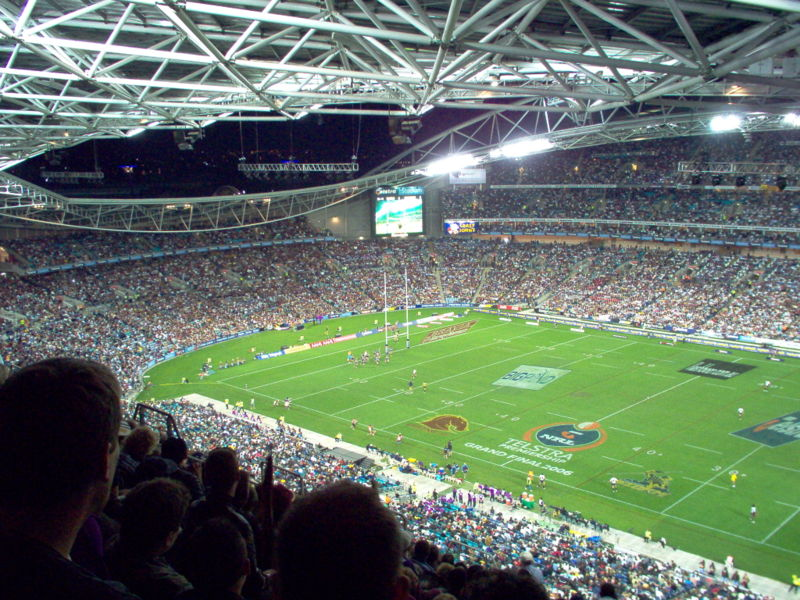
\includegraphics[width=0.6\textwidth]{images/football.jpg}

Credit: MDM, Wikimedia Commons
\end{center}

\end{frame}


\begin{frame}
\frametitle{Motivation}

\begin{itemize}
\item This is a `fun'\footnote{Your mileage may vary.}
lecture where each year I try to predict the NRL
(Rugby League tournament based in Australia) grand final result using Bayesian
statistics. \pause
\item It is somewhat related to logistic regression.\pause
\item The model will start off relatively simple, but will eventually
become a hierarchical model.
\end{itemize}
\end{frame}

\begin{frame}
\frametitle{NRL}

\begin{itemize}
\item The NRL is the (Australian) National Rugby League tournament (it also
includes the New Zealand Warriors).\pause
\item There are 17 teams in the competition.\pause
\item The grand final will be played on Sunday, between the teams:
TBD.
\end{itemize}
\end{frame}

\end{document}

